\documentclass[tikz,border=5pt]{standalone}
\usetikzlibrary{positioning, fit, backgrounds}

\begin{document}

% Compile this locally using pdflatex. 
% It will generate a PDF with transparent background.
% You can convert the PDF to SVG or PNG (con sfondo trasparente) per Canva.

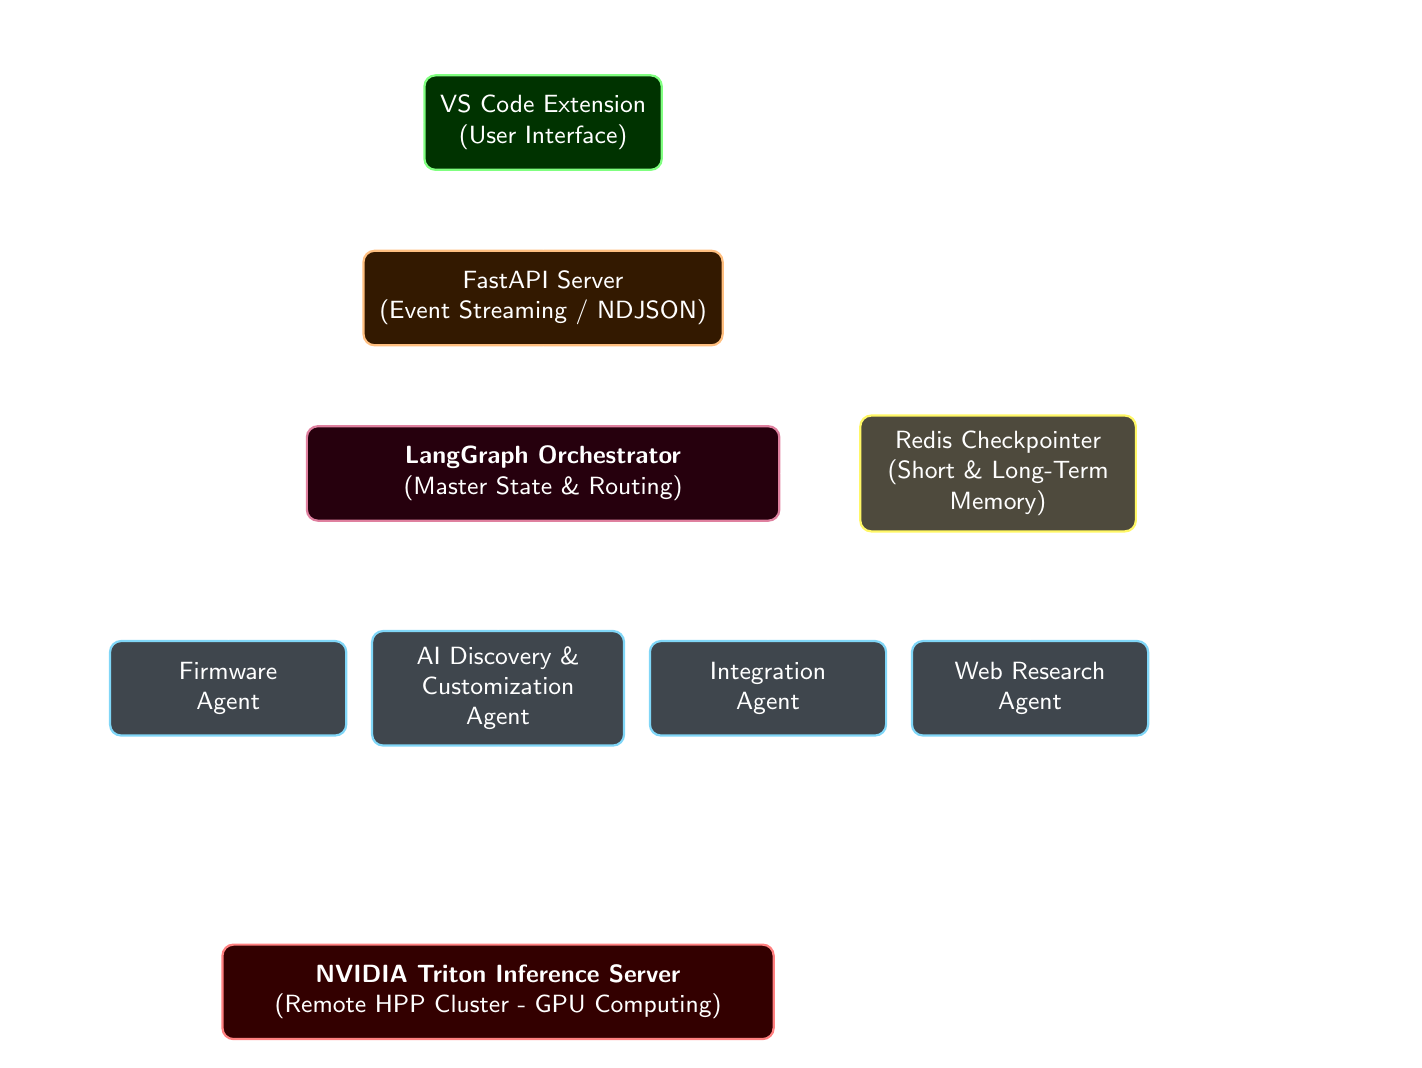
\begin{tikzpicture}[
        scale=1.0, transform shape,
        node distance=1.5cm and 1.8cm,
        % Testo di default bianco per leggibilità su sfondo scuro Canva
        every node/.style={font=\sffamily\small, text=white},
        % Stile box: Sfondo molto scuro (es. mix 20% colore principale e 80% nero), bordo luminoso
        box/.style={draw, rounded corners, minimum width=3cm, minimum height=1.2cm, align=center, thick, inner sep=0.2cm},
        % Frecce chiare e visibili
        arrow/.style={->, thick, >=stealth, draw=white!85},
        % Etichette dei layer (L1, L2, ecc)
        layerlabel/.style={font=\sffamily\footnotesize\bfseries, text=white!60, align=center}
    ]

    % --- LAYER 1: Presentation ---
    % fill=green!20!black -> verde molto scuro, draw=green!50 -> bordo verde acceso
    \node[box, fill=green!20!black, draw=green!50] (vscode) {VS Code Extension\\(User Interface)};
    \node[left=0.5cm of vscode, align=center, text width=2.5cm, text=white!95] (user) {Developer\\Commands/Chat};
    \draw[arrow] (user) -- (vscode);

    % --- LAYER 2: API & Comm ---
    \node[box, below=1cm of vscode, fill=orange!20!black, draw=orange!50] (fastapi) {FastAPI Server\\(Event Streaming / NDJSON)};

    % --- LAYER 3: Orchestration ---
    \node[box, below=1cm of fastapi, minimum width=6cm, fill=purple!20!black, draw=purple!50, text=white] (langgraph) {\textbf{LangGraph Orchestrator}\\(Master State \& Routing)};

    % --- LAYER 4: State & Memory ---
    \node[box, right=1cm of langgraph, minimum width=3.5cm, fill=yellow!20!black, draw=yellow!60] (redis) {Redis Checkpointer\\(Short \& Long-Term\\Memory)};

    % --- Agentic Workflows (part of Orchestration Layer) ---
    \node[box, below=1.5cm of langgraph, xshift=-4cm, fill=cyan!20!black, draw=cyan!50, text width=2.4cm] (fw_agent) {Firmware\\Agent};
    \node[box, right=0.3cm of fw_agent, fill=cyan!20!black, draw=cyan!50, text width=2.8cm] (ai_agent) {AI Discovery \&\\Customization\\Agent};
    \node[box, right=0.3cm of ai_agent, fill=cyan!20!black, draw=cyan!50, text width=2.4cm] (int_agent) {Integration\\Agent};
    \node[box, right=0.3cm of int_agent, fill=cyan!20!black, draw=cyan!50, text width=2.4cm] (web_agent) {Web Research\\Agent};

    % --- LAYER 5: Compute & Inference Backend ---
    \node[box, below=2.5cm of ai_agent, minimum width=7cm, fill=red!20!black, draw=red!50] (triton) {\textbf{NVIDIA Triton Inference Server}\\(Remote HPP Cluster - GPU Computing)};

    % --- Connections ---
    \draw[arrow, <->] (vscode) -- node[right, text=white!85] {HTTP / REST} (fastapi);
    \draw[arrow, <->] (fastapi) -- (langgraph);

    % Redis connection
    \draw[arrow, <->] (langgraph.east) -- (redis.west);

    % Downward arrow to horizontal bus, then fan-out to agents
    \coordinate (bus) at ([yshift=-0.75cm]langgraph.south);
    \draw[arrow] (langgraph.south) -- (bus);
    \draw[white!85, thick] (fw_agent.north |- bus) -- (web_agent.north |- bus);
    \draw[arrow] (bus -| fw_agent.north) -- (fw_agent.north);
    \draw[arrow] (bus -| ai_agent.north) -- (ai_agent.north);
    \draw[arrow] (bus -| int_agent.north) -- (int_agent.north);
    \draw[arrow] (bus -| web_agent.north) -- (web_agent.north);

    % Inference dashed lines
    \draw[arrow, <->, dashed] (ai_agent.south) -- node[left, text=white!85] {LLM/AI Inference} (triton.north -| ai_agent.south);

    % Routing Inference: straight line between AI Discovery and Integration Agent
    \path (ai_agent.east) -- (int_agent.west) coordinate[midway] (mid_ai_int);
    \draw[arrow, <->, dashed] (langgraph.south -| mid_ai_int) -- node[right, near end, text=white!85] {Routing Inference} (triton.north -| mid_ai_int);

    % === LAYER LABELS ===
    \node[layerlabel, above=0.1cm of vscode] {L1: IDE Layer};
    \node[layerlabel, right=0.3cm of fastapi] {L2: API Gateway};
    \node[layerlabel, left=1cm of langgraph] {L3: Orchestration};
    \node[layerlabel, anchor=west] at ([xshift=0.3cm]redis.east) {L4: State \& Memory};
    \node[layerlabel, left=0.5cm of triton] {L5: Inference};

\end{tikzpicture}
\end{document}
